\documentclass{article}
	\usepackage[ansinew]{inputenc}
	\usepackage{ae}
	\usepackage{SIunits}
	\usepackage{amsmath}
	\usepackage{graphicx}
	\usepackage{xcolor}
\begin{document}

	\section*{Grupo de simetrias do tri�ngulo equil�tero}

	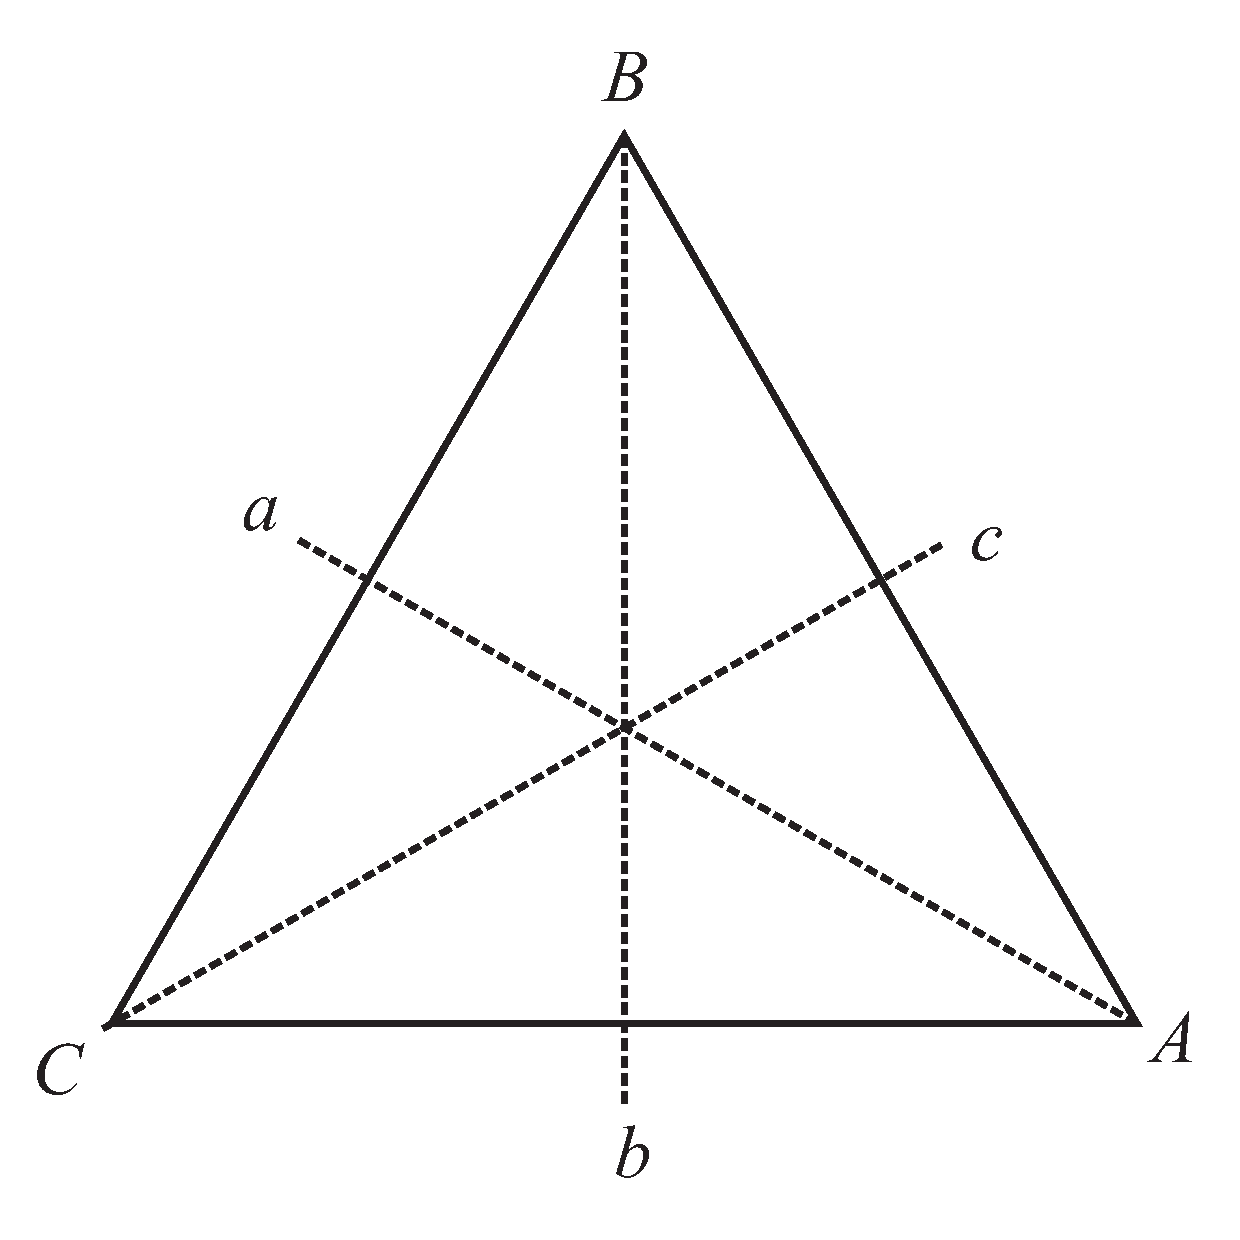
\includegraphics[width=0.3\textwidth]{triangle.pdf}

	\begin{itemize}
	
		\item Elementos do grupo $G$:
			\begin{itemize}
				\item[$i$] Identidade
				\item[$a$] Reflex�o $\overline{aA}$
				\item[$b$] Reflex�o $\overline{bB}$
				\item[$c$] Reflex�o $\overline{cC}$
				\item[$d$] Rota��o de \unit{120}{\degree} (ao redor do centro do tri�ngulo)
				\item[$e$] Rota��o de \unit{240}{\degree} (ao redor do centro do tri�ngulo)
			\end{itemize}
	
		\item	Tabela de multiplica��o:\par
			\begin{tabular}{c|cccccc}
				    & $i$ & $a$ & $b$ & $c$ & $d$ & $e$ \\
				    \hline
				$i$ & $i$ & $a$ & $b$ & $c$ & $d$ & $e$ \\
				$a$ & $a$ & $i$ & $d$ & $e$ & $b$ & $c$ \\
				$b$ & $b$ & $e$ & $i$ & $d$ & $c$ & $a$ \\
				$c$ & $c$ & $d$ & $e$ & $i$ & $a$ & $b$ \\
				$d$ & $d$ & $c$ & $a$ & $b$ & $e$ & $i$ \\
				$e$ & $e$ & $b$ & $c$ & $a$ & $i$ & $d$ \\
			\end{tabular}

		\item A ordem (quantidade de elementos) do grupo � $g = 6$.
		
		\item A tabela de multiplica��o n�o � sim�trica. Logo, o grupo \emph{n�o} � abeliano. Isto tamb�m pode ser deduzido da ordem do grupo ($g = 6$): como $g$ n�o � um n�mero primo, o grupo n�o pode ser abeliano.
		
		\item $g = 1\cdot2\cdot3$. Portanto, subgrupos t�m 1, 2 ou 3 elementos apenas.
		
		\item Classes de equival�ncia:
			\begin{itemize}
				\item[] $\mathcal{C}_1 = \{a,b,c\}$ 
				\item[] $\mathcal{C}_2 = \{d,e\}$
				\item[] $\mathcal{C}_3 = \{i\}$
			\end{itemize}
	
		\item Subgrupos f�ceis de achar: $\{i\},\quad \{i,a\},\quad \{i,b\},\quad \{i,c\},\quad \{i,d,e\}.$
		\item O subgrupo $\{i\}$ � invariante.
		\item O subgrupo $\{i,d,e\} \equiv A$ � invariante.
		\item Os subgrupos $\{i,a\}$, $\{i,b\}$ e $\{i,c\}$ \emph{n�o} s�o invariantes.
		\item	Grupo fator $G|A = \{A,aA\} = \{A, bA\} = \{A, cA\}$.
		\item $G$ � isom�rfico com $S_3$, fazendo a seguinte correla��o:
			\begin{itemize}
				\item[] $i \to \text{Identidade}$
				\item[] $a \to (12)$
				\item[] $b \to (23)$
				\item[] $c \to (13)$
				\item[] $d \to (123)$
				\item[] $e \to (321)$
			\end{itemize}
			
		\item Uma representa��o bidimensional desse grupo � a seguinte (\textcolor{red}{verificando}):
			\item[] $D(i) =
				\begin{pmatrix}
					1 & 0 \\
					0 & 1
				\end{pmatrix}$
			\item[] $D(a) =
				\begin{pmatrix}
					-1/2        & -\sqrt{3}/2 \\
					-\sqrt{3}/2 & 1/2
				\end{pmatrix}$
			\item[] $D(b) =
				\begin{pmatrix}
					1 & 0 \\
					0 & -1
				\end{pmatrix}$
			\item[] $D(c) =
				\begin{pmatrix}
					-1/2       & \sqrt{3}/2 \\
					\sqrt{3}/2 & 1/2
				\end{pmatrix}$
			\item[] $D(d) =
				\begin{pmatrix}
					-1/2        & \sqrt{3}/2 \\
					-\sqrt{3}/2 & -1/2
				\end{pmatrix}$
			\item[] $D(e) =
				\begin{pmatrix}
					-1/2        & -\sqrt{3}/2 \\
					\sqrt{3}/2 & -1/2
				\end{pmatrix}$
		\end{itemize}

\end{document}